% RESULTADOS-------------------------------------------------------------------

\chapter{RESULTADOS}
\label{chap:resultados}

Nesse capitulo serão discutido, os resultados globais obtidos com o desenvolvimento do protótipo e, mostrado um teste comparativo entre dois \textit{codecs} de video testados com a biblioteca \textit{FFmpeg}.\par

\subsection{Resultados Globais}
\label{subsec:resglobais}

De modo geral, o protótipo se comportou conforme o esperado. A captura de movimento da cabeça do operador funcionou de maneira satisfatória e os motores respondem sem atrasos perceptíveis (que representassem desconforto ao operador). Entretanto, em determinados momentos, os motores apresentaram movimentos bruscos, como se estivessem perdendo coordenadas. Posteriormente, com o auxilio da função \textit{CAMDEMO},  descobriu-se que o comportamento inesperado dos motores, acontecia devido a algum tipo de incompatibilidade com o pino \textit{GPIO} usado para acionar o motor horizontal. O servo passou a ser acionado por outro pino \textit{GPIO} e o problema foi resolvido.\par

Durante os testes com o \textit{driver} PWM criado, ilustrado na \autoref{fig:pwmtestcircuit}, foi possível observar que o motor responde de forma estável para uma faixa de frequência, e não só em 50Hz. Testes foram feitos com a frequência variando entre aproximadamente 44Hz e 62Hz. Entretanto, é muito sensível quanto a variação da largura dos pulsos, apresentando um comportamento errático quando a largura do pulso oscilava.\par

Conforme citado na \autoref{sec:assemprototipo}, a fonte de tensão dos motores foi separada da fonte de tensão do \textit{Raspberry Pi} para evitar o ruido causado pelos motores. Contudo, foi possível notar um comportamento indesejado, que acontece esporadicamente, ao acionar os motores. Em determinados momentos, após acionar os motores, foi possível notar uma queda de tensão de até 0,5V na linha de 5V por alguns segundos, causando a desconexão da rede sem fio e consequentemente impossibilitando receber as coordenadas enviadas pelo MCM. Capacitores foram adicionados a linha de 5V, na tentativa de resolver o problema porem, a queda de tensão persistiu. Por ser intermitente, é provável que o comportamento indesejado seja causado por algum tipo de mau contato na \textit{breadboard}. \par

O sistema de envio de imagens precisa ser optimizado. Talvez um dispositivo de captura com mais qualidade, como o módulo de câmera oficial do \textit{Raspberry Pi}, que possui um drive especifico implementado em \textit{hardware}, represente uma melhoria no sistema global de captura e envio de imagens para o celular.\par

Os eventos de detecção de posição, gerados pela API do \textit{Android}, ocorrem em um tempo especificado pelo desenvolvedor. Para identificar esse tempo, levou-se em consideração a responsividade necessária para os motores e o uso de banda de dados. Quanto menor o intervalo de tempo entre os eventos, maior a resolução do movimento,  consumo de banda de dados e custo computacional. Para chegar-se a um valor adequado, testes práticos foram feitos variando-se o intervalo de eventos entre 10 e 500 milissegundos. Chegou-se a conclusão que valores entre 30 e 100 milissegundos são satisfatórios.\par

\begin{figure}[H]
	\centering
	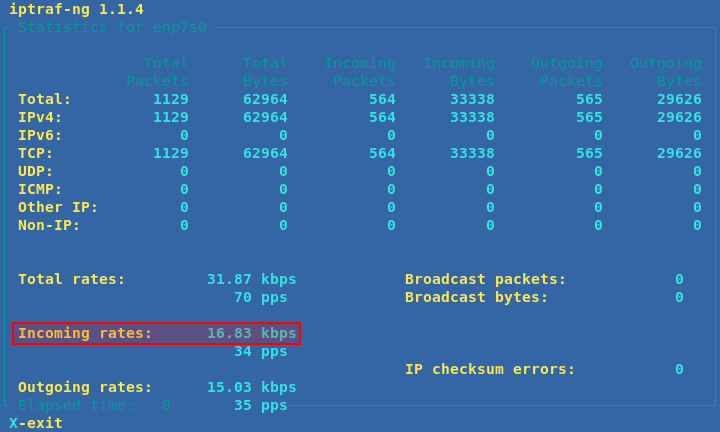
\includegraphics[width=1\textwidth]{figuras/consumo_banda_unfiltered.png}
	\caption{Consumo dos recursos de rede durante o recebimento de coordenadas sem o filtro.}
	\label{fig:consumo_banda_coord_unfiltered}
\end{figure}

\begin{figure}[H]
	\centering
	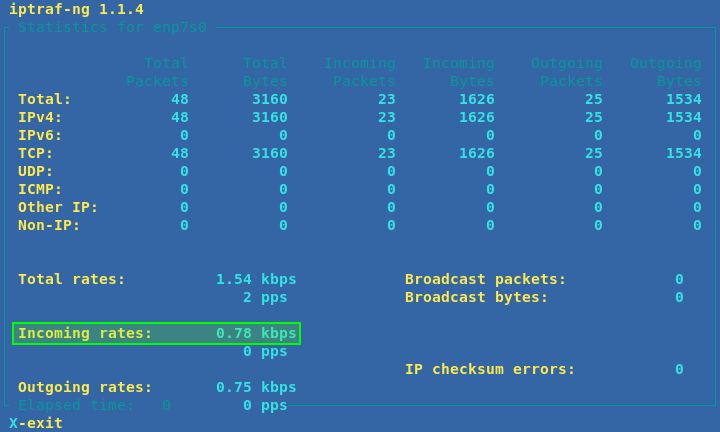
\includegraphics[width=1\textwidth]{figuras/consumo_banda_filtered.png}
	\caption{Consumo dos recursos de rede durante o recebimento de coordenadas com o filtro.}
	\label{fig:consumo_banda_coord_filtered}
\end{figure}

A banda de dados consumida pelo envio de coordenadas, foi minimizado pela aplicação de um filtro, que compara a última coordenada válida com a que será enviada, conforme explicado no final da \autoref{subsec:assemmodcapmov}. Desse modo somente as modificações de posição são enviadas ao MCM. O resultado da aplicação desse filtro pode ser visualizado comparando-se a \autoref{fig:consumo_banda_coord_unfiltered} e a \autoref{fig:consumo_banda_coord_filtered}. Os testes de rede rodaram por aproximadamente 10 segundos com o MCM acoplado à cabeça do operador em posição de repouso (movimento mínimo).\par

A \autoref{fig:consumo_banda_video} mostra o consumo de banda de dados quando o MCC está transmitindo o vídeo capturado pela câmera. Vale notar que a soma de recursos de rede, consumidos pelas funções de envio de coordenada e de transmissão de vídeo, não ultrapassam a banda disponível de 100Mbps. Portanto afastando a possibilidade de esgotamento de banda de dados, que impediria a comunicação correta entre os módulos.\par

\begin{figure}[H]
	\centering
	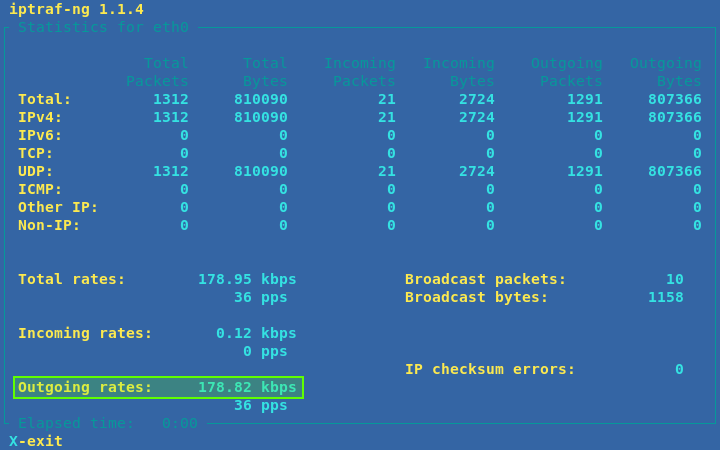
\includegraphics[width=1\textwidth]{figuras/consumo_banda_camera.png}
	\caption{Consumo dos recursos de rede durante o envio de imagem da câmera.}
	\label{fig:consumo_banda_video}
\end{figure}

\subsection{Comparação Entre \textit{codecs}}
\label{subsec:compcodecs}

Dentre os testes realizados com alguns dos \textit{codecs} de vídeo compatíveis com o FFmpeg, os que mais chamaram atenção e que representaram um ganho considerável, em relação ao custo computacional, foram os \textit{codecs} \textbf{h264\_omx} e \textbf{h264}, implementados em hardware e software respectivamente.
Comparando-se a \autoref{fig:top_ffmpeg_h264} e a \autoref{fig:top_ffmpeg_h264_omx}, obtidas da interface do gerenciador de tarefas \textit{top}, fica claro que a implementação de \textit{codecs} via hardware traz um ganho, em tempo de processador e quantidade de memoria \textit{RAM} alocada, considerável. Existe um ganho de aproximadamente 28\% em tempo de processador e 35\% em uso de memoria \textit{RAM}. Uma parte do uso de recursos nas duas figuras está relacionada ao processo de \textit{streaming}, implementada via software. Como o \textit{streaming} é o mesmo para as duas comparações, não existe inconsistência na comparação.

\begin{figure}[H]
	\centering
	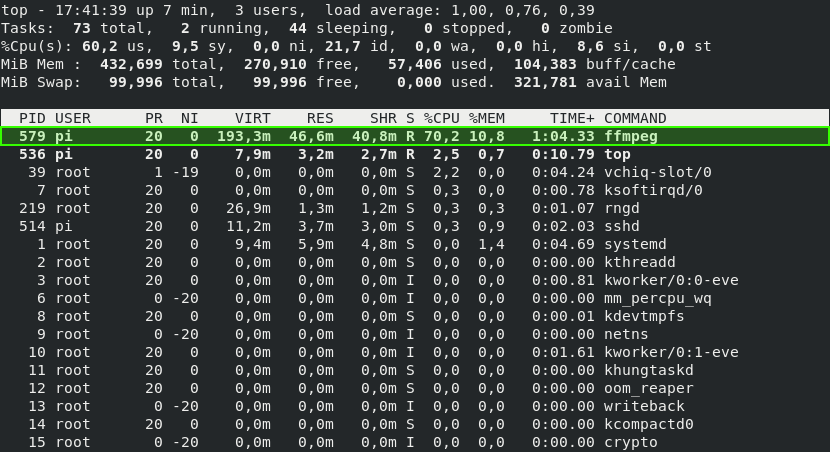
\includegraphics[width=1\textwidth]{figuras/top_ffmpeg_h264_omx.png}
	\caption{Consumo de recursos de hardware pelo FFmpeg usando o codec h264\_omx, implementado em hardware.}
	\label{fig:top_ffmpeg_h264_omx}
\end{figure}

\begin{figure}[H]
	\centering
	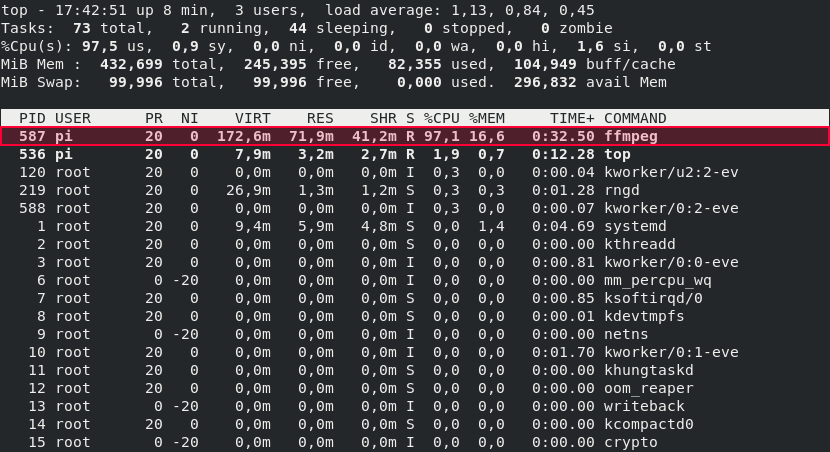
\includegraphics[width=1\textwidth]{figuras/top_ffmpeg_h264.png}
	\caption{Consumo de recursos de hardware pelo FFmpeg usando o codec h264, implementado em software.}
	\label{fig:top_ffmpeg_h264}
\end{figure}
